\documentclass[11pt, letterpaper, twocolumn, fleqn]{article}
\usepackage[margin=0.5in]{geometry}
\usepackage[utf8]{inputenc}
\usepackage{amsmath,amssymb,amsthm,graphicx, textcomp, siunitx}

\graphicspath{ {./images/} }

\let\oldemptyset\emptyset
\let\emptyset\varnothing

\sisetup{output-exponent-marker=\ensuremath{\mathrm{e}}}

\begin{document}
\renewcommand{\labelenumi}{\alph{enumi}.}
\renewcommand{\labelenumii}{(\arabic{enumii})}
\renewcommand{\qedsymbol}{$\blacksquare$}

\widowpenalties 1 10000
\raggedbottom
\pagestyle{headings}

\paragraph{7.1.1}
\begin{enumerate}
  \item $G$ has 7 edges so it has a total degree of $2 \cdot 7 = 14$.
  \item The neighbors of 5 are $\{6,1,2,3,4\}$
  \item 6's only neighbor is 5, so its degree is 1.
  \item $\{2,5\}$ is the set of vertices adjacent to 3.
  \item $G$ is not a regular graph because not all vertices have the same degree, for example: $deg(5) \neq deg(6)$
  \item Yes, the set $\{1,2,5\}$ form the graph $K_3$ that is a subgraph of $G$.
  \item No, $K_4$ is not a subgraph of $G$ because there are no 4 vertices that are all connected to each other.
\end{enumerate}

\paragraph{7.1.4}
\begin{enumerate}
  \item There are $3 \cdot 4 = 12$ edges in $K_{3,4}$. $K_{3,4}$ is not a regular graph because the vertices on the left side have 4 neighbors each and the vertices on the right have 3 neighbors each.
  \item There are 10 edges in $K_5$. $K_5$ is a regular graph because all the vertices have a degree of 4.
  \item $n=3$ is the largest n such that $K_n = C_n$. 
\end{enumerate}

\paragraph{7.2.2}
\begin{enumerate}
  \item 
  \begin{align*}
    &\fbox{1} \rightarrow \fbox{2}\fbox{5} \\
    &\fbox{2} \rightarrow \fbox{1}\fbox{3}\fbox{5}\\
    &\fbox{3} \rightarrow \fbox{2}\fbox{5}\\
    &\fbox{4} \rightarrow \fbox{5}\\
    &\fbox{5} \rightarrow \fbox{1}\fbox{2}\fbox{3}\fbox{4}\fbox{6}\\
    &\fbox{6} \rightarrow \fbox{5}
  \end{align*}
  \item 
  $$\begin{bmatrix}
    0 & 1 & 0 & 0 & 1 & 0 \\
    1 & 0 & 1 & 0 & 1 & 0 \\
    0 & 1 & 0 & 0 & 1 & 0 \\
    0 & 0 & 0 & 0 & 1 & 0 \\
    1 & 1 & 1 & 1 & 0 & 1 \\
    0 & 0 & 0 & 0 & 1 & 0
  \end{bmatrix}$$
\end{enumerate}

\paragraph{7.4.1}
\begin{enumerate}
  \item There are 4 connected components of $G$:
    $$\{a,b,c\},\{e,d\},\{f,h,i,j\},\{g\}$$
    
  \item There are no connected vertices in $G$. Therefore, there are 5 connected components of $G$:
    $$\{a\},\{b\},\{c\},\{d\},\{e\}$$
    
  \item There is 1 connected component of $G$:
    $$\{a,b,c,d,e,f\}$$
    
\end{enumerate}

\paragraph{7.4.2}
\begin{enumerate}
  \item The vertex connectivity is 1. If vertex 6 is removed, there are no connections between $\{1,2,3,4\}$ and $\{5,7,8\}$.
  
  The edge connectivity is 2. If edges $\{\{1,2\},\{1,4\}\}$ are removed, then vertex 1 id disconnected from the graph. Removing any single edge will not disconnect the graph.
  
  \item The vertex connectivity is 1. If vertex 3 is removed, then vertex 1 is disconnected from the graph. 
  
  The edge connectivity is also 1 because if the edge $\{1,3\}$ is removed, then vertex 1 is disconnected from the graph.
\end{enumerate}

\paragraph{7.4.4}
\begin{enumerate}
  \item If every pair of vertices in $G$ are 2-edge-connected, no more and no less, then by definition the graph is actual a cycle $C_n$ on $|V|$ vertices. From here it is plain to see that removing any 1 edge will not disconnect the graph and that removing 2 edges that don't share any vertices will.
  
  \item Yes the property is transitive. Let there be a cycle $C$ with vertices $V = \{v,w,y\}$. All vertices in a cycle are 2-edge-connected, therefore $v$ and $w$ are 2 edge connected, $w$ and $y$ are two edge connected, and $v$ and $y$ are two edge connected.
\end{enumerate}

\paragraph{7.5.1}
\begin{enumerate}
  \item An Euler circuit for the graph is 
    $$\langle a,b,c,f,a,c,d,e,b,f,d,a \rangle$$
    
  \item The graph does not have an Euler circuit because 2 vertices have an odd degree, $\{b,f\}$.
\end{enumerate}

\paragraph{7.6.1}
\begin{enumerate}
  \item $\{p,l,h,m\}$ are ancestors of vertex $n$.
  \item $\{f,g,e,d,a,b,c\}$ are all descendants of vertex i.
  \item $\{j,q,n,e,a,b,c,g\}$ are the leaves of the tree.
  \item Vertex $d$ is on level 3.
  \item The height of the tree is 5.
  \item $\{o,n,a,b,c\}$ are the level 4 vertices.
  \item 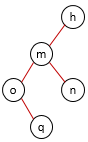
\includegraphics{761g}
  \item $\{l,k\}$ are siblings of vertex i.
\end{enumerate}

\end{document}
